% !TEX root = thesis.tex
%\newcommand{\baselineEvalFigure}{
\begin{figure}[t]
    \centering
    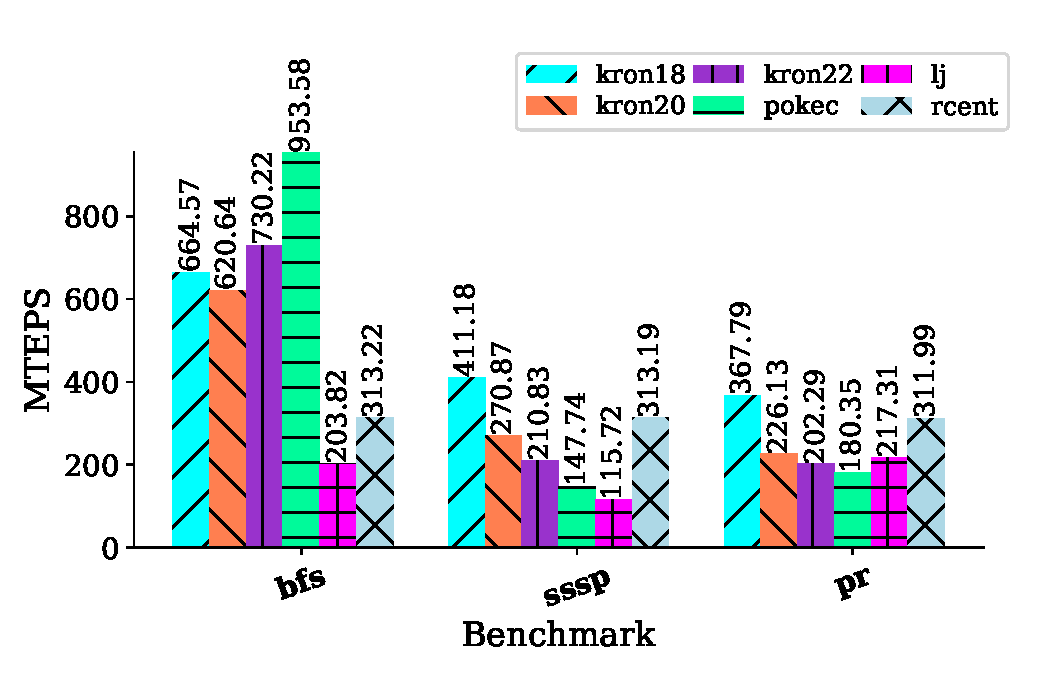
\includegraphics[scale = 0.5]{graphit-figures/baseline.pdf}
    \caption{Baseline code generation results for each benchmark in the dense pull direction with no manycore specific optimizations.}
    \label{pap:generals:sec:eval:fig:baseline}
\end{figure}
}

\newcommand{\pushEvalFigure}{
\begin{figure}[t]
    \centering
    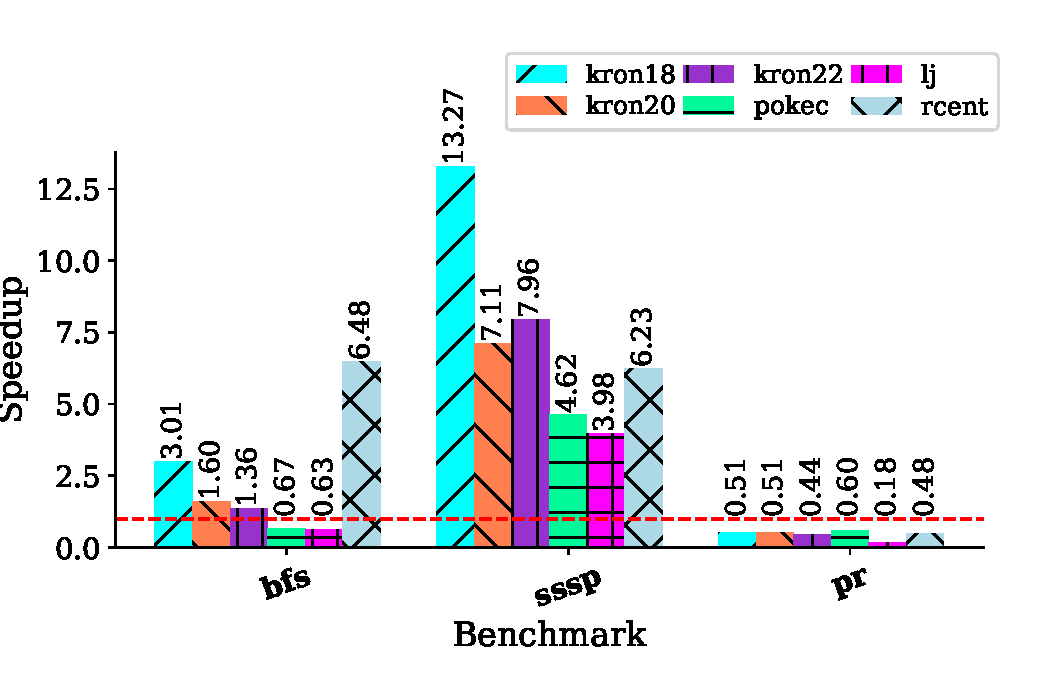
\includegraphics[scale = 0.5]{graphit-figures/push.pdf}
    \caption{Baseline code generation results for each benchmark in the push direction with no manycore specific optimizations.}
    \label{pap:generals:sec:eval:fig:push}
\end{figure}
}

\newcommand{\edgeSpeedupFigure}{
\begin{figure}[t]
    \centering
    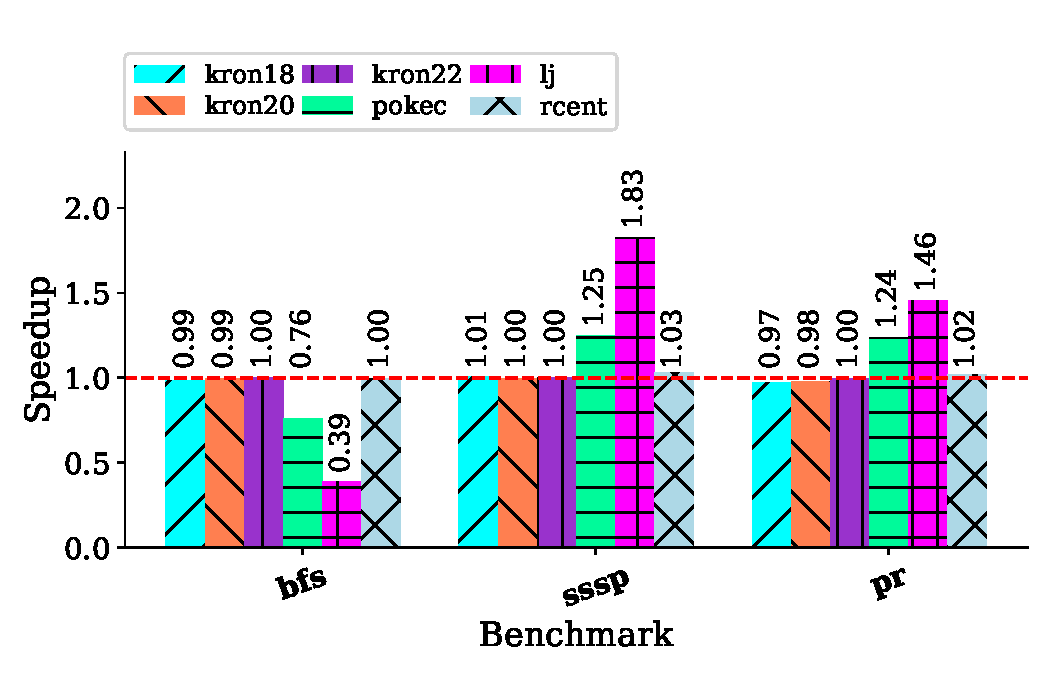
\includegraphics[scale = 0.5]{graphit-figures/edge.pdf}
    \caption{Speedup results for edge based optimization over the baseline dense pull implementation for each benchmark.}
    \label{pap:generals:sec:eval:fig:edge}
    \vspace{-2mm} 
\end{figure}
}

\newcommand{\blockBFSFigure}{
\begin{figure}[t]
    \centering
    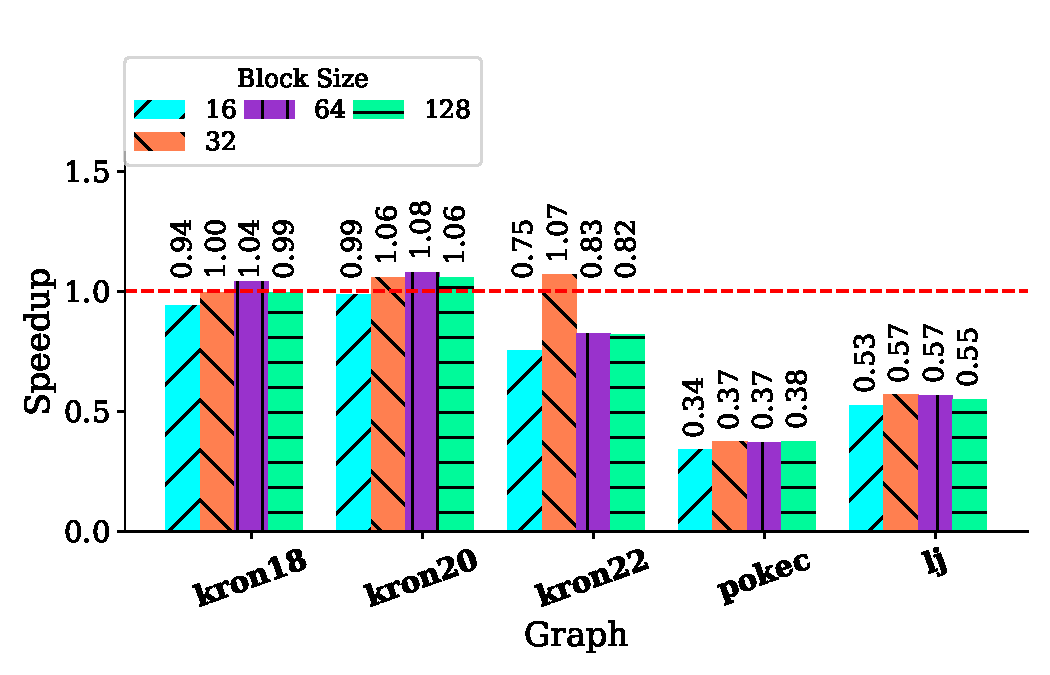
\includegraphics[scale = 0.5]{graphit-figures/bfs-block.pdf}
    \caption{MTEPS results for varying block sizes using the blocked access method on BFS.}
    \label{pap:generals:sec:eval:fig:bfsblock}
\end{figure}
}

\newcommand{\blockSSSPFigure}{
\begin{figure}[t]
    \centering
    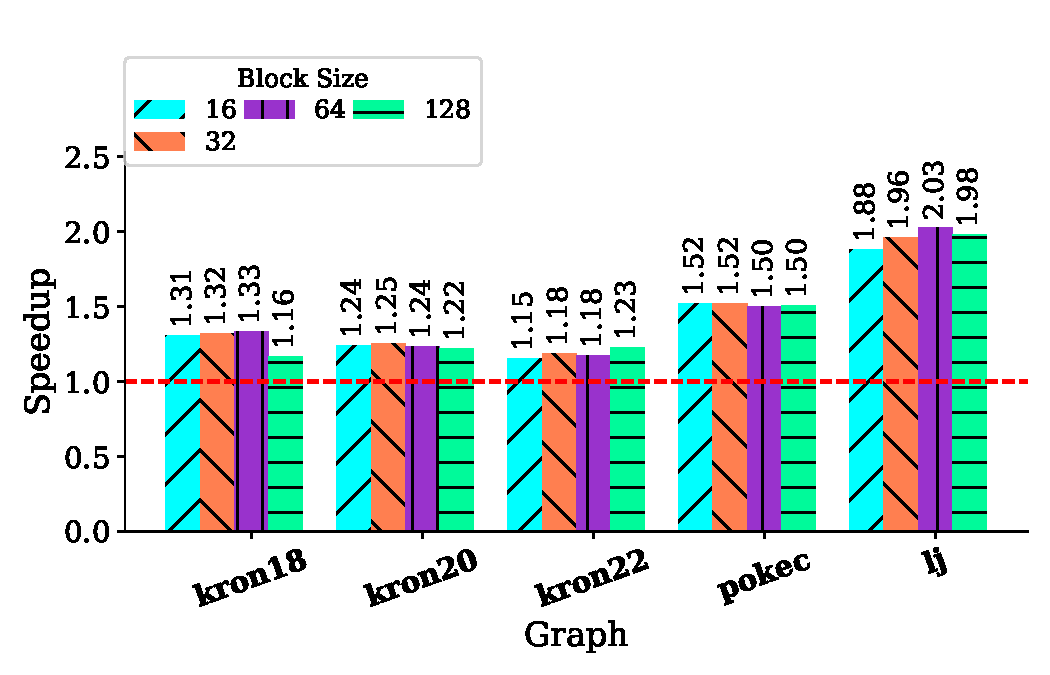
\includegraphics[scale=0.5]{graphit-figures/sssp-block.pdf}
    \caption{Speedup results for varying block sizes using the blocked access method on SSSP. Speedup is calculated over the baseline pull direction implementation.}
    \label{pap:generals:sec:eval:fig:ssspblock}
\end{figure}
}

\newcommand{\cacheBFSFigure}{
\begin{figure}[t]
    \centering
    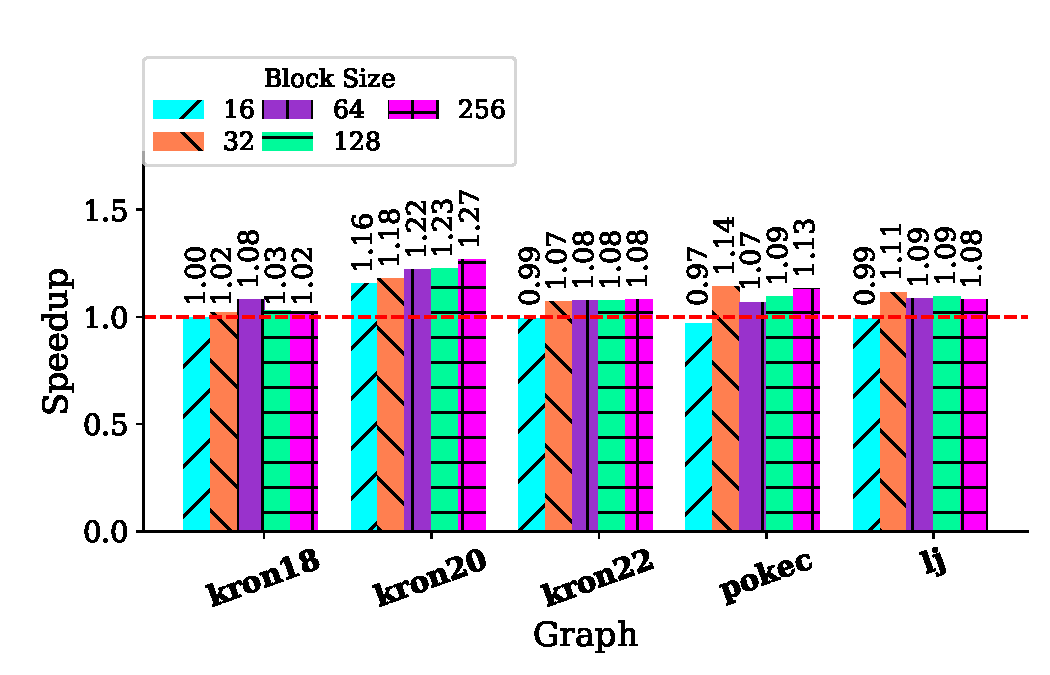
\includegraphics[scale = 0.5]{graphit-figures/bfs-cache.pdf}
    \caption{MTEPS results for varying work block sizes using the manycore aware vertex partitioning scheme on BFS.}
    \label{pap:generals:sec:eval:fig:bfscache}
\end{figure}
}

\newcommand{\cacheSSSPFigure}{
\begin{figure}[t]
    \centering
    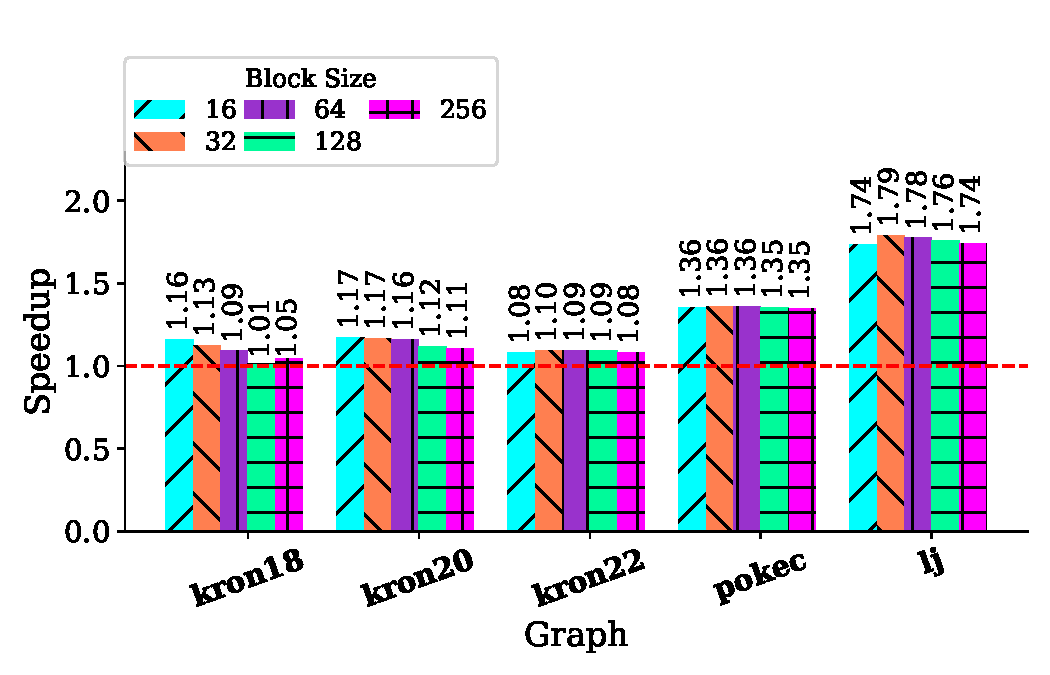
\includegraphics[scale=0.5]{graphit-figures/sssp-cache.pdf}
    \caption{Speedup results for varying work block sizes using the manycore aware vertex partitioning scheme on SSSP. Speedup is calculated over the baseline pull direction implementation.}
    \label{pap:generals:sec:eval:fig:ssspcache}
\end{figure}
}

\newcommand{\allBlockedFigure}{
\begin{figure}[t]
    \centering
    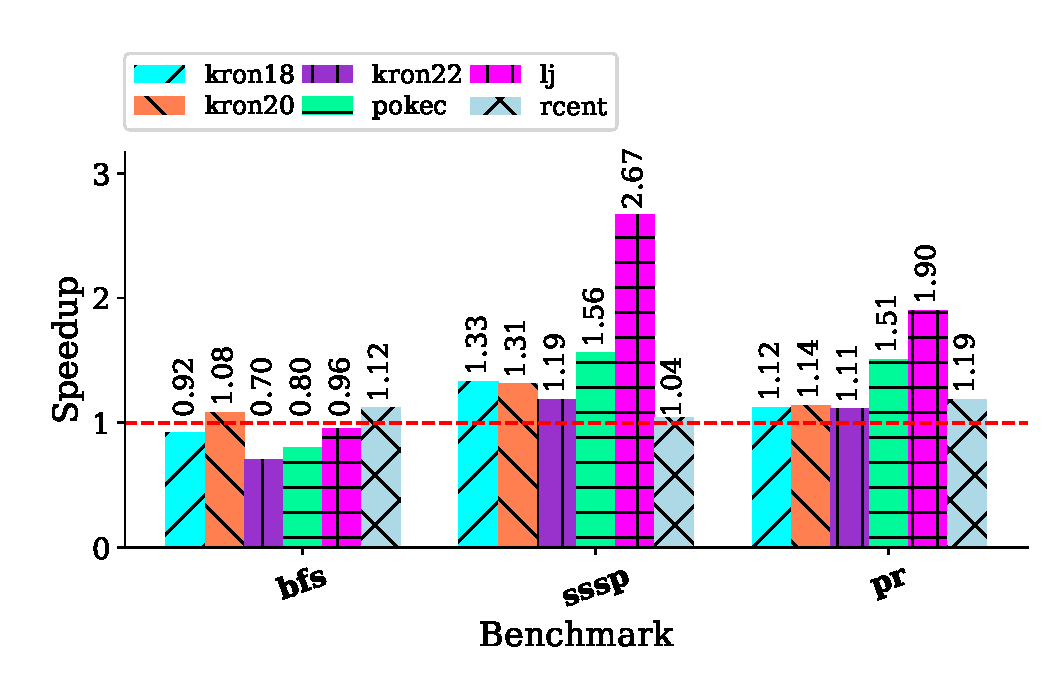
\includegraphics[scale = 0.5]{graphit-figures/all-blocked.pdf}
    \caption{Blocked access method speedup results for each benchmark. Speedup is calculated over the baseline pull direction implementation.} %For each graph and benchmark, block sizes of 16, 32, 64, and 128 elements were tested and the best performing block size is reported here.
    \label{pap:generals:sec:eval:fig:blocked}
\end{figure}
}

\newcommand{\allAlignedFigure}{
\begin{figure}[t]
    \centering
    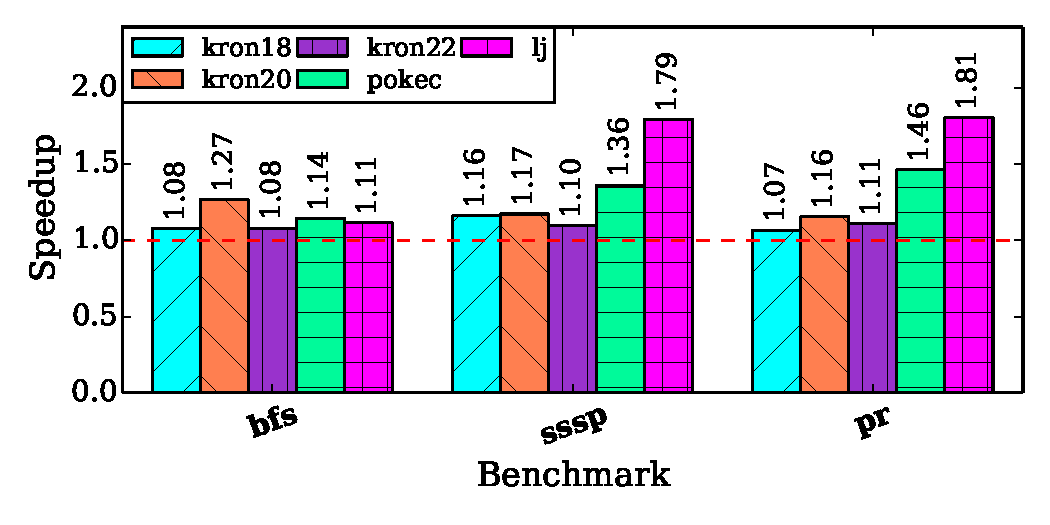
\includegraphics[scale = 0.5]{graphit-figures/align.pdf}
    \caption{Alignment-based partitioning speedup results for each benchmark. Speedup is calculated over the baseline pull direction implementation.} %For each graph and benchmark, work group sizes of 16, 32, 64, 128, and 256 vertices were tested and the best performing work group size is reported here.
    \label{pap:generals:sec:eval:fig:aligned}
    \vspace{-2mm} 
\end{figure}
}

%I am not sure if this is the best way to present an overview of results or if we need it. 
\newcommand{\overviewResultsTable}{
\begin{table}[]
\centering
\begin{tabular}{lrcl}
%\hline
\toprule
\textbf{Benchmark} & \textbf{Graph} & \textbf{MTEPS} & \textbf{Optimization} \\ \midrule
 \multirow{5}{*}{BFS}& kron18 & 457.09 & Cache-Aligned \pull \\ %\cline{2-4}
 & kron20 & 296.32 & Cache-Aligned \pull \\ %cline{2-4}
 & kron22 & 241.95 & Cache-Aligned \pull \\ %\cline{2-4}
 & pokec & 148.02 &  Cache-Aligned \pull\\ %\cline{2-4}
 & lj & 304.36 & Cache-Aligned \pull \\ \hline
 \multirow{5}{*}{PR}& kron18 & 412.34 & Blocked \pull \\ %\cline{2-4}
 & kron20 & 261.35 & Cache-Aligned \pull \\ %\cline{2-4}
 & kron22 & 224.88 & Blocked \pull \\ %\cline{2-4}
 & pokec & 272.57 & Blocked \pull \\ %\cline{2-4}
 & lj & 413.06 & Blocked \pull \\ \hline
 \multirow{5}{*}{SSSP}& kron18 & 467.08 & Cache-Aligned \pull \\ %\cline{2-4}
 & kron20 & 364.36& Baseline \push \\ %\cline{2-4}
 & kron22 & 404.27 & Baseline \push \\ %\cline{2-4}
 & pokec & 149.17 & Cache-Aligned \pull \\ %\cline{2-4}
 & lj & 268.87 & Cache-Aligned \pull \\ %\hline
 \bottomrule
\end{tabular}
\caption{Table containing best MTEPS results across all benchmarks and input graphs. The optimizations used to achieve these results are also listed above.}
\label{pap:generals:sec:eval:tab:overview}
\end{table}
}

\newcommand{\relatedMTEPSTable}{
\begin{table}[]
\centering
\begin{tabular}{cllll}
%\hline
\toprule
 \textbf{Source} & \textbf{Platform} & \textbf{Benchmark} & \textbf{Graph}  & \textbf{MTEPS} \\ \midrule
 \cite{slota2015high}& Xeon Phi MIC & CC & LJ (22) & 240 \\ %\hline
 \cite{slota2015high}& Xeon Phi MIC & CC & Flickr (19) & 140\\ %\hline
 %Galois \cite{aasawat2018well}& Ivy Bridge & PR & LJ (22) & 207.67 \\ \hline
 \cite{khorasani2014cusha} & GTX780 & BFS & LJ (22) & 272.4 \\ %\hline
 \cite{zhong2013medusa}& C2050 & BFS & KKT (21) & 351.5 \\ %\hline
 \cite{yang2019graphblast}& k40c & SSSP & LJ (22) & 334.2 \\ %\hline
 \cite{wang2016gunrock} & k40c & SSSP & LJ (22) & 217.9 \\
 \bottomrule

\end{tabular}
\caption{Performance results in MTEPS from other graph processing frameworks. The benchmark CC is strongly connected components.}
\label{sec:related:tab:mteps}
\vspace{-1mm} 
\end{table}
}
\newcommand{\graphInfoTable}{
\begin{table}[]
\centering
\begin{tabular}{c|c|c|c}
%\hline
 \textbf{Name} & \textbf{Scale} & \textbf{\# Vertices} & \textbf{\# Edges} \\ \hline %\hline
 kron18 & 18 & 262,144 & 4,194,304 \\ \hline
 kron20 & 20 & 1,048,576 & 16,777,216 \\ \hline
 kron22 & 22 & 4,194,304 & 67,108,864 \\ \hline
 pokec & 20.5 & 1,632,803 & 30,622,564 \\ \hline
 livejournal (lj) & 22 & 3,997,962 & 34,681,189 \\ %\hline
\end{tabular}

\caption{The vertex and edge information for each of the graphs used in our evaluation. We use synthetic \kron graphs used in the Graph500 benchmark and two real world graphs.}
\label{sec:eval:tab:graphs}
\end{table}
}

%\subsection{Evaluation} \label{sec:eval}
%In this subsection, we evaluate the performance of our GraphIt code generation backend and its optimizations outlined in Sections~\ref{sec:method} and~\ref{sec:method:sub:baseline}.
%We compare the performance of our generated code to a CPU baseline and evaluate the performance of each of the optimizations we outlined in Section~\ref{sec:method}. 

\section{Experimental Setup}

%\graphInfoTable
\begin{table}[]
    \centering
    \begin{tabular}{c|c|c|c}
    %\hline
     \textbf{Name} & \textbf{Scale} & \textbf{\# Vertices} & \textbf{\# Edges} \\ \hline %\hline
     kron18 & 18 & 262,144 & 4,194,304 \\ \hline
     kron20 & 20 & 1,048,576 & 16,777,216 \\ \hline
     kron22 & 22 & 4,194,304 & 67,108,864 \\ \hline
     pokec & 20.5 & 1,632,803 & 30,622,564 \\ \hline
     livejournal (lj) & 22 & 3,997,962 & 34,681,189 \\ %\hline
    \end{tabular}
    
    \caption{The vertex and edge information for each of the graphs used in our evaluation. We use synthetic \kron graphs used in the Graph500 benchmark and two real world graphs.}
    \label{sec:eval:tab:graphs}
\end{table}

Host software executes natively on an Intel Xeon Gold 6254 CPU.
The host libraries interface directly with the simulator environment using the SystemVerilog DPI interface.
We compile all generated C++ code using the GNU Compiler Collection (GCC) with ``-O2''.

\paragraph{Manycore Architecture}
% We evaluate our compiler using detailed RTL simulation of our manycore architecture.
We model a manycore system running at 1GHz with 16 columns and 8 rows for a total of 128 cores.
The machine has a 512KB 8-way set associative LLC with 128-byte lines.
The memory system uses two HBM2 memory channels.
We model the HBM2 memory system with DRAMSim3\cite{li2019dramsim3},  a timing accurate simulator for modeling DRAM.
We use detailed, cycle-accurate RTL simulation to model our processor cores, network on chip, and LLC.
Our simulation environment includes SystemVerilog bind modules for collecting performance metrics such as instruction and cycle counts.
The RTL for this manycore has been validated in silicon, and this configuration occupies approximately 3.5 mm$^2$ of die area. 
%We also collect other profiling statistics such as processor stalls and opcode histograms.

\paragraph{Benchmarks} We evaluate our compiler on three common graph benchmarks: Breadth-First Search (BFS), Single Source Shortest Path (SSSP), and PageRank (PR). 
BFS has a high memory access to computation ratio and is a component of many graph algorithms.
PageRank computes the importance of each vertex in the graph, and unlike BFS, spends most of its time performing computation on the entire graph.
PR also users floating point operations.
%SSSP operates on a weighted graph.
SSSP operates on a larger subset of the edges during execution and tends to be more sensitive to load balancing.
We implement the Bellman-Ford variant of SSSP for our evaluation.

We implement all of these benchmarks in GraphIt and generate manycore code using our GraphIt code generation backend.
Due to the time costs of simulation, we do not run all iterations of our benchmarks. 
For BFS and SSSP, we run one iteration from the middle of execution with a maximal root node selected as the initial frontier.
For PR, we run one iteration from the beginning of execution.



\paragraph{Graphs} We use two types of graphs in our evaluation: synthetic \kron graphs used in the Graph500 benchmark~\cite{murphy2010graph500} and real-world, social network graphs.
\kron graphs follow a power law distribution in order to simulate the small world property often seen in real world graphs~\cite{leskovec2010kronecker}.
We generate three \kron graphs of varying size. 
%We generate weighted and unweighted versions of each of these graphs for use with our three benchmarks.
We use two real-world graphs: pokec~\cite{pokec} and livejournal~\cite{lj}.
All of the graphs we use and their properties are shown in Table~\ref{sec:eval:tab:graphs}.


\section{Results}
%\baselineEvalFigure
\begin{figure}[t]
    \centering
    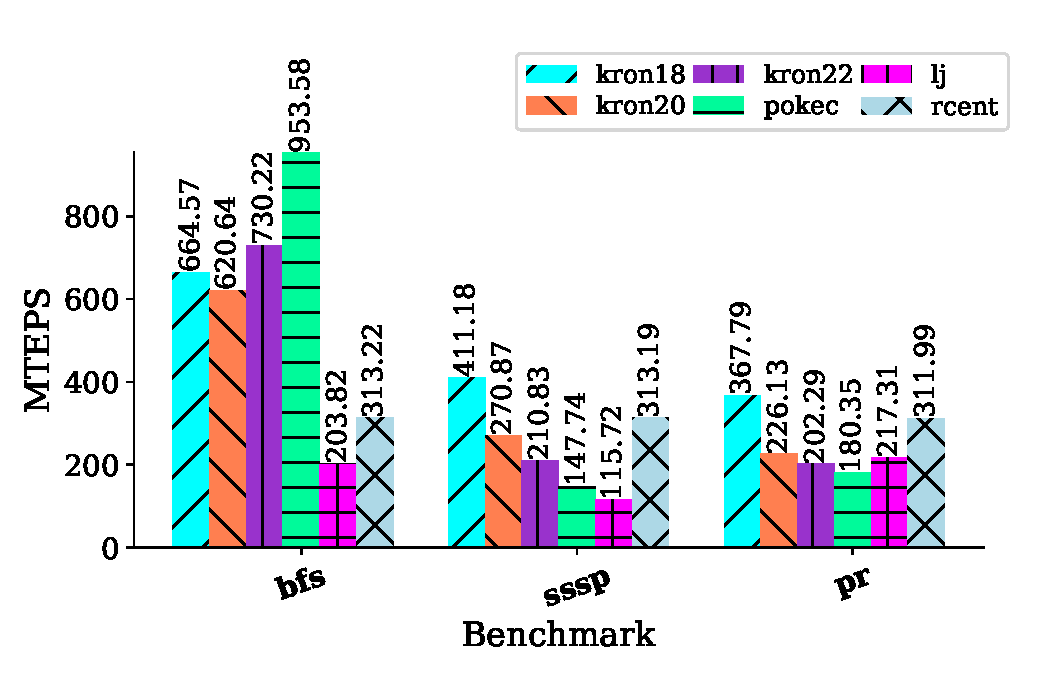
\includegraphics[scale = 0.5]{graphit-figures/baseline.pdf}
    \caption{Baseline code generation results for each benchmark in the dense pull direction with no manycore specific optimizations.}
    \label{pap:generals:sec:eval:fig:baseline}
\end{figure}

%\todo[inline]{Results intro}
To evaluate our code generator, we first present performance results for the unoptimized benchmarks. 
We then explore the performance trade-offs and benefits for each of the optimizations described in Section~\ref{sec:method}.

\subsection{Baseline}
 
%\pushEvalFigure
\begin{figure}[t]
    \centering
    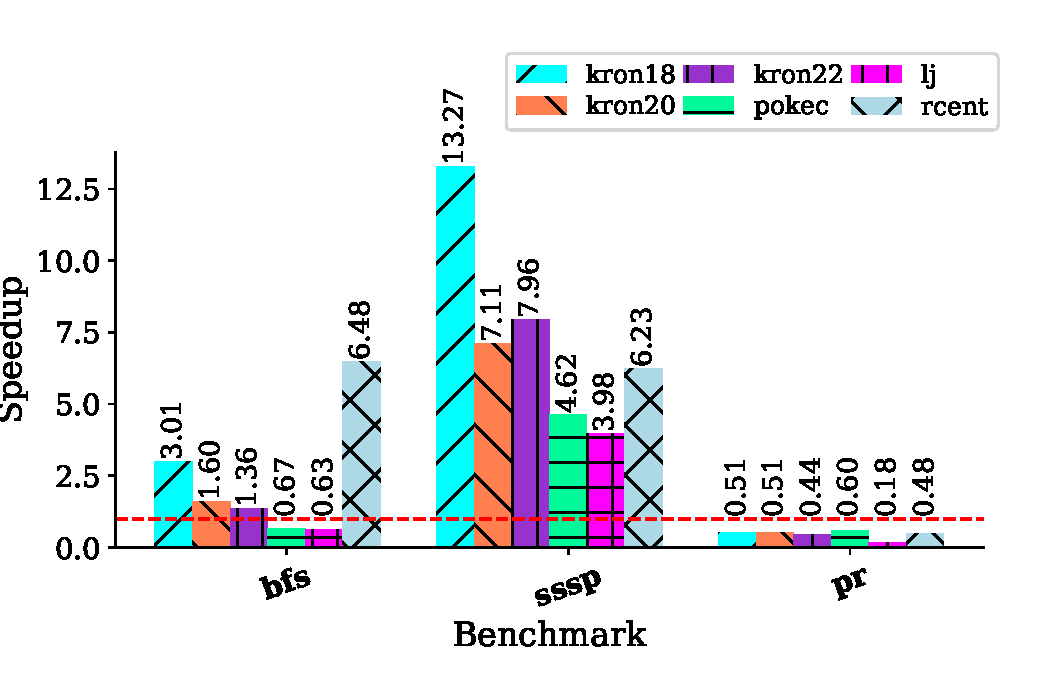
\includegraphics[scale = 0.5]{graphit-figures/push.pdf}
    \caption{Baseline code generation results for each benchmark in the push direction with no manycore specific optimizations.}
    \label{pap:generals:sec:eval:fig:push}
\end{figure}
To establish a baseline, we examine the performance of the code produced by our backend without any added optimizations.
To evaluate performance, we calculate the traversed edges per second (TEPS) for each iteration of each benchmark using the cycle counts that we obtain from simulation.

Figures~\ref{pap:generals:sec:eval:fig:baseline} and~\ref{pap:generals:sec:eval:fig:push} show our initial performance results for the manycore code generated by our backend without added optimizations in the \pull~and \push~directions respectively as described in Section~\ref{sec:method:sub:baseline}.
Across all of these, we see a geometric mean of 214 MTEPS in the \pull~direction and 104 MTEPS in the \push~direction. 
This decrease in performance in the \push~direction is expected as the iterations we examine for BFS and SSSP have very dense frontiers that benefit from traversing in the \pull~direction.
In all three benchmarks, we see the highest performance on the \kron scale 18 graph.
This is most likely due to the relative small size of the graph and the large amount of parallelism and memory bandwidth present on the manycore architecture.
 
BFS has a very high memory access to compute ratio, so the number of reads greatly affects the performance.
Because we use iterations from the middle of execution, a large number of vertices do not need to be visited in the \pull~direction that would need to be visited in the \push~direction. %because they have already been visited in previous iterations.
We see an average increase in performance of 3.6$\times$ just from traversing in the \pull~direction instead of \push. 
 
We see less clear results with SSSP.
For SSSP we observe better performance in the \pull~direction on the real world graphs, but not on the two larger \kron graphs.
From our simulation results, we are able to see that these \kron graphs make better use of the LLCs and issue fewer reads to HBM in the \push~direction, accounting for the improvement in performance. 
 
Interestingly, PageRank sees a performance improvement across all graphs in the \pull~direction.
Unlike BFS, PageRank must visit all vertices in all iterations regardless of traversal direction.
When we examined our simulation results, we saw that the \pull~direction issued fewer read requests to HBM which most likely accounts for the difference in performance. 
 
% \cpuResultsTable
  
% To contextualize these results, we include parallel CPU results in MTEPS for each benchmark and input graph in Table~\ref{pap:cgp21:sec:eval:tab:cpuresults}.
% We generate the parallel C++ code for these tests using the GraphIt CPU backend and run with OpenMP.
% We run these tests on a 4 socket, 72 core, 144 hyperthread, Intel Xeon Gold 6254 CPU running at 3.10 GHz with 25 MB LLC and 3 TB of DDR4 running at 2666MHz.
% It is challenging to provide a direct performance comparison between the two architectures because they are optimized for different goals.
% The Xeon is a high-performance server class CPU with relatively high area and power budgets.
% By contrast, the manycore is designed to be a flexible and low-cost substrate for parallel compute.
%\todo[inline]{somehow expand here and explain why we don't do more of a comparison. maybe also mention that we are simulating only a portion of the entire manycore}
% Manycore is optimized for area and power vs the Xeon optimized for performance.
% We are simulating a quarter of a real chip due to the constraints of our detailed simulation infrastructure.
%The Xeon is a server class CPU with a latency-optimized memory system and relatively high area and power budgets.
%The manycore uses only a tiny fraction of the die area of a Xeon and is designed to achieve best performance per Watt.
 
\subsection{Blocking}
%\blockSSSPFigure
\begin{figure}[t]
    \centering
    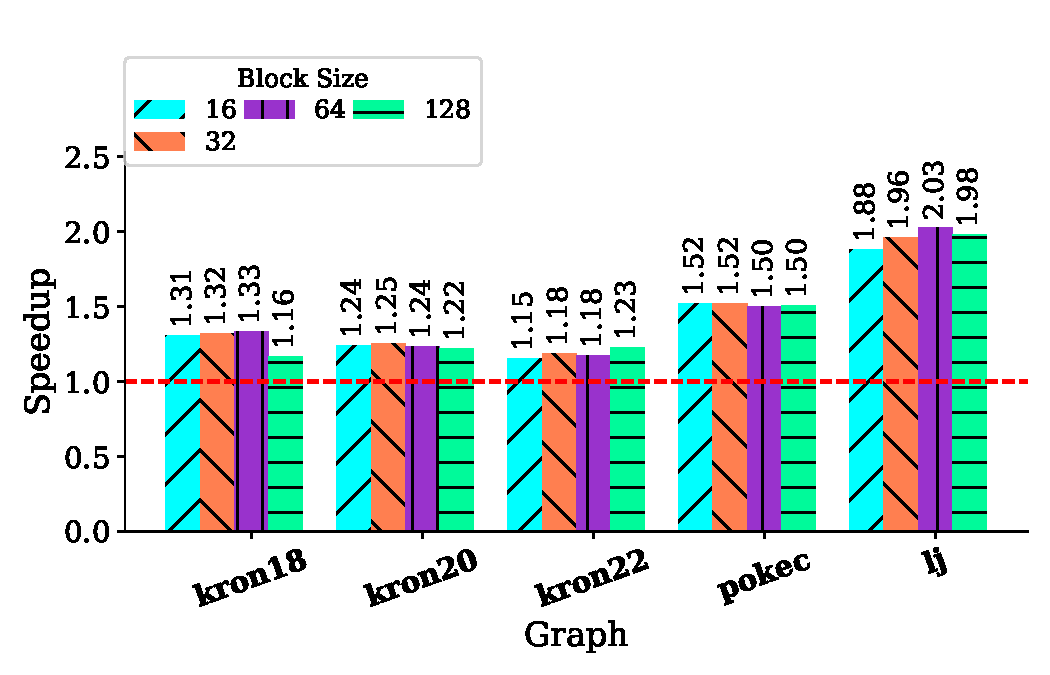
\includegraphics[scale=0.5]{graphit-figures/sssp-block.pdf}
    \caption{Speedup results for varying block sizes using the blocked access method on SSSP. Speedup is calculated over the baseline pull direction implementation.}
    \label{pap:generals:sec:eval:fig:ssspblock}
\end{figure}
 
%\allBlockedFigure
\begin{figure}[t]
    \centering
    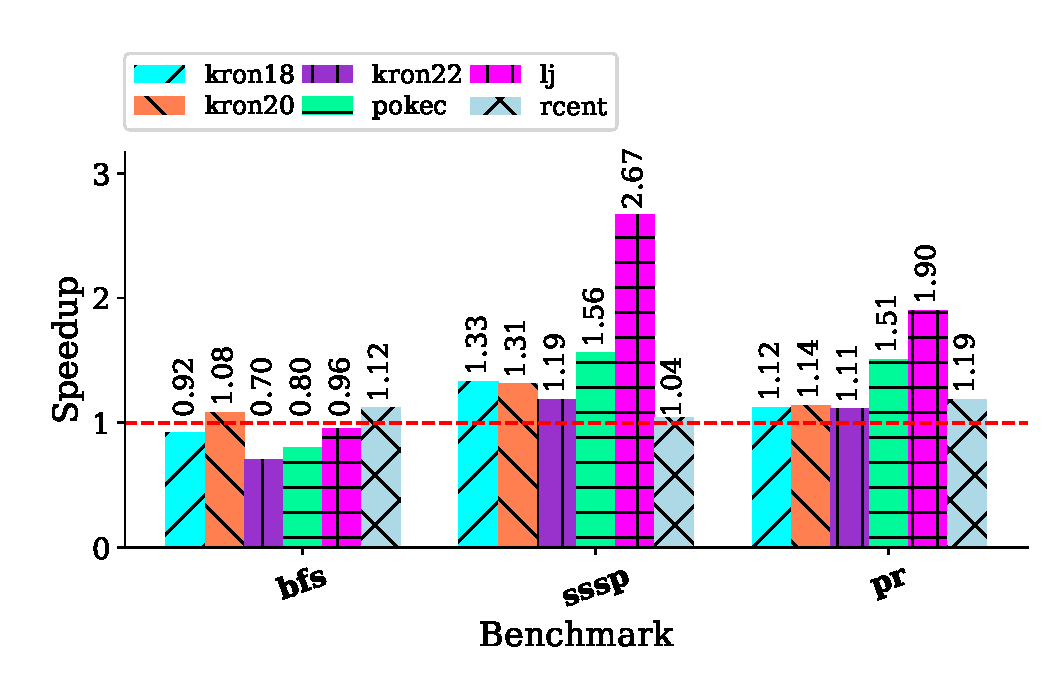
\includegraphics[scale = 0.5]{graphit-figures/all-blocked.pdf}
    \caption{Blocked access method speedup results for each benchmark. Speedup is calculated over the baseline pull direction implementation.} %For each graph and benchmark, block sizes of 16, 32, 64, and 128 elements were tested and the best performing block size is reported here.
    \label{pap:generals:sec:eval:fig:blocked}
\end{figure}
 
Figure~\ref{pap:generals:sec:eval:fig:ssspblock} shows the performance benefit of the blocking optimization across different block sizes on the SSSP benchmark in the \pull~direction. Results for block sizes of 16, 32, 64, and 128 elements are shown.
Speedup is normalized to the baseline performance of SSSP in the \pull~direction without any optimizations.
 
Interestingly, we do not see much variation in speedup across different block sizes. 
Livejournal and \kron 18 see the most speedup with a block size of 64, pokec and \kron 20 see optimal performance with block size 32, and a block size of 128 is optimal for \kron 22. 
We observe that the optimal block size appears to be input graph dependent for the other benchmarks we studied as well. 
 
Figure~\ref{pap:generals:sec:eval:fig:blocked} shows the speedup for each benchmark when using the blocked access method. 
Again, speedup is normalized to the baseline performance of each benchmark in the \pull~direction.
In this figure, the optimal block size for each input graph and benchmark is used in computing the speedup. 
Blocking provides a mean speedup of 1.21$\times$ and a maximum speedup of 2.01$\times$. 
 
Blocking is primarily motivated by the microarchitecture's ability to hide memory load latency.
The prefetching effect from blocking can yield significant performance improvement, but it also provides the effect of data caching.
Even if the data is used once, the prefetching effect can yield significant performance improvement. 
We observe the most speedup with SSSP because it traverses more edges than BFS and benefits most from prefetching.
We see the least speedup from blocking with BFS and see performance degredation on the pokec and livejournal graphs.
The \pull~direction for BFS traverses the fewest edges of the three workloads thanks to a filter condition on destination vertices.
This means that much of the prefetched data is never used, and the additional memory reads become overhead.

Overall, we find that our blocking optimization provides performance improvement in all but two cases. 
Blocking reduces stalls from memory system requests and improves the hit rate of the LLC. We find, however, that it does not have a large impact on DRAM stalls.
Making use of the low-latency scratchpad memory and coalescing accesses most improve performance on benchmarks that traverse more edges in the graph. 
 
\subsection{Work Partitioning}
 
%\cacheSSSPFigure
\begin{figure}[t]
    \centering
    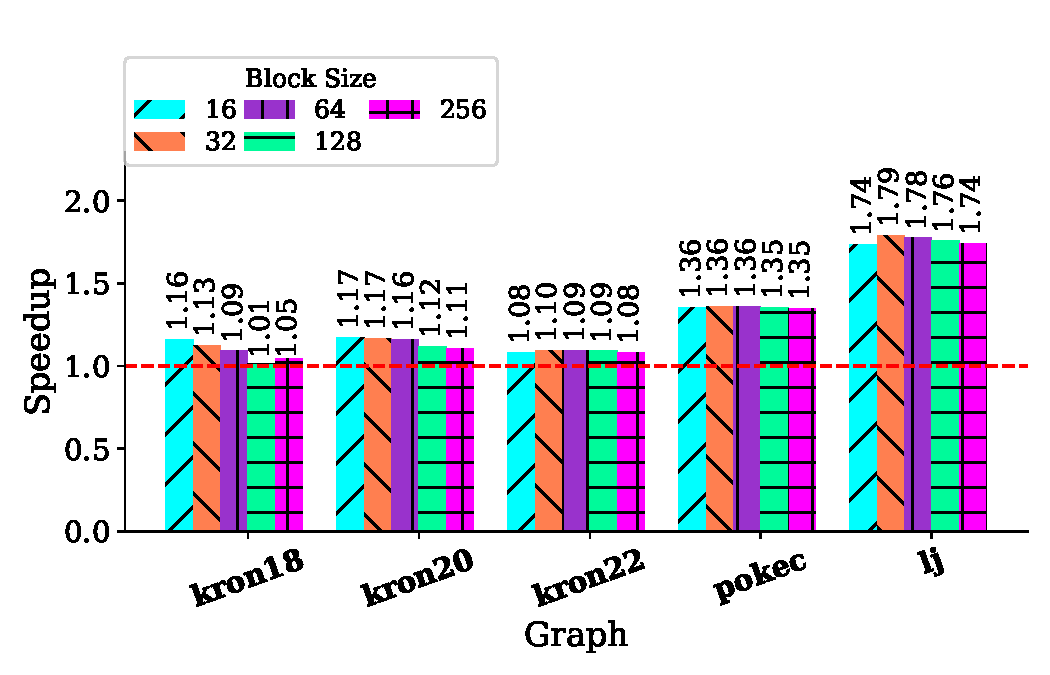
\includegraphics[scale=0.5]{graphit-figures/sssp-cache.pdf}
    \caption{Speedup results for varying work block sizes using the manycore aware vertex partitioning scheme on SSSP. Speedup is calculated over the baseline pull direction implementation.}
    \label{pap:generals:sec:eval:fig:ssspcache}
\end{figure}
 
%\allAlignedFigure
\begin{figure}[t]
    \centering
    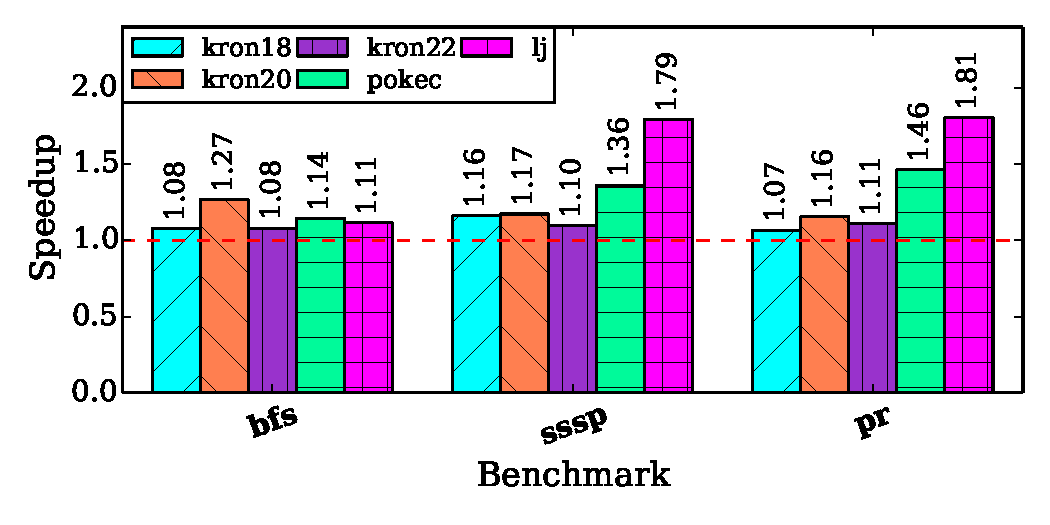
\includegraphics[scale = 0.5]{graphit-figures/align.pdf}
    \caption{Alignment-based partitioning speedup results for each benchmark. Speedup is calculated over the baseline pull direction implementation.} %For each graph and benchmark, work group sizes of 16, 32, 64, 128, and 256 vertices were tested and the best performing work group size is reported here.
    \label{pap:generals:sec:eval:fig:aligned}
    \vspace{-2mm} 
\end{figure}
 
Figure~\ref{pap:generals:sec:eval:fig:ssspcache} shows the performance benefit of alignment-based partitioning across different work block sizes.
Speedup is calculated over the baseline SSSP \pull~implementation. 
Similarly to the blocked access method results, we find that the optimal work block size for alignment-based partitioning is input graph and benchmark dependent. 
A work block size of 16 is optimal for \kron 18 and 20, livejournal and \kron22 see the best performance with a block size of 32, and pokec sees the most speedup with a block size of 64.
 
Figure~\ref{pap:generals:sec:eval:fig:aligned} shows the speedup for each benchmark when using alignment-based partitioning over the baseline vertex partitioning scheme. The optimal work block size for each input graph and benchmark is used to calculate speedup. 
We observe a performance improvement in all input graph and benchmark combinations with an average speedup of 1.25$\times$ and a maximum speedup of 1.8$\times$. 
 
Alignment-based partitioning aims to make better use of the memory system on the manycore. 
By assigning smaller working sets to each core, there is less contention in the LLCs and all benchmarks achieve higher cache hit rates. 
Improving the LLC hit rate decreases the total amount of memory that needs to be read from HBM and decreases the amount of time spent waiting on outstanding memory requests.
 
 
%\edgeSpeedupFigure
\begin{figure}[t]
    \centering
    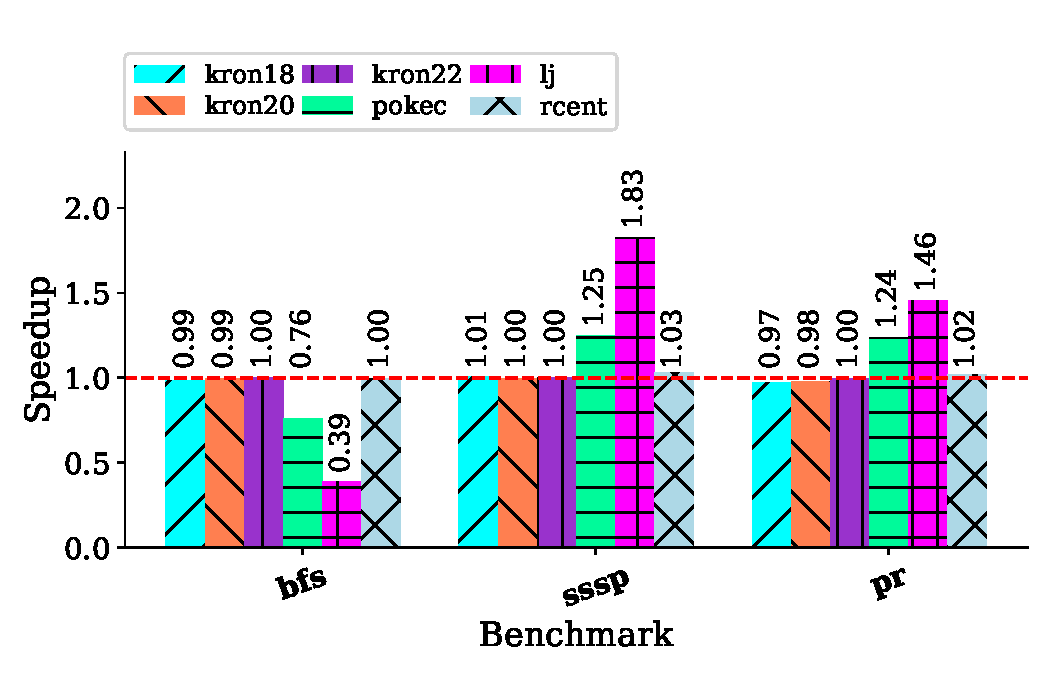
\includegraphics[scale = 0.5]{graphit-figures/edge.pdf}
    \caption{Speedup results for edge based optimization over the baseline dense pull implementation for each benchmark.}
    \label{pap:generals:sec:eval:fig:edge}
    \vspace{-2mm} 
\end{figure}
 
Figure~\ref{pap:generals:sec:eval:fig:edge} shows the performance of edge-aware vertex partitioning relative to the baseline vertex-based partitioning on all benchmarks in the \pull~direction. 
We achieve a speedup in five of the benchmark and input graph combinations with a maximum speedup of 1.5$\times$.
In the cases where performance degraded, we observe an average slowdown 11.7\%. 
This scheduling optimization relies heavily on the structure of the input graph and the algorithm, so these results are somewhat expected.
 
Overall, while we see performance improvements with edge-aware vertex-based partitioning on some benchmarks, we find that alignment-based partitioning provides the most performance improvement in all cases. 
Despite its workload balancing benefits, edge-aware partitioning does not account for the manycore specific properties of the memory system.
Because the memory is the main bottleneck of graph algorithms, the alignment-based scheme which explicitly takes into consideration the properties of the manycore's memory system is ideal. 
 
% \section{Discussion}\label{sec:discussion}
 %\overviewResultsTable
 

% \section{Discussion}\label{sec:discussion}
% %\todo[inline]{(emily) need to reconfigure figure~\ref{fig:overallresults} to group by optimization and by scale of graph (instead of just on optimization like it is now). also need to make sure labels are shown for bars that go above y-axis max}
% \begin{figure}
%     \centering
%     \includegraphics[width=\textwidth]{figures/optimization-speedups_no16.pdf}
%     \caption{Speedups for all of the optimizations we explored in our evaluation. Speedups are calculated over the serial CPU baseline. Speedup is also reported for the parallel CPU implementation over the serial baseline.}
%     \label{fig:overallresults}
% \end{figure}

% Figure~\ref{fig:overallresults} shows an overview of all of the results we presented in Section~\ref{sec:eval}. 
% It shows the speedup for each optimization over the serial CPU baseline in terms of traversed edges per second (TEPS). We observe speedups in 28 of the 30 different cases shown in the figure. We achieve a mean speedup of 3.8$\times$ across optimizations and only see a slowdown of 10\% in the worst case. 

% We see the largest speedups with our blocked \push and blocked \pull implementations.
% This is not surprising, as all of our benchmarks are limited by DRAM, and blocking is an optimization that makes better use of the memory system.
% %This is not surprising, as all of our benchmarks are limited by the memory system performance, and blocking is a memory system optimization.
% By adding blocking, we are able to coalesce read accesses to vertex data, and with the \pull direction, we are also able to batch some of the writes.
% In addition, we able to make use of explicitly managed, low-latency scratchpad memory in our blocked access method. 
% The blocked access method improves the memory system performance of our benchmarks by targeting a key performance limiter of graph algorithms.

% We observe our greatest individual speedups on the \push direction implementations of SSSP. 
% In both the blocked and unblocked implementations, we see very large speedups with the scale 18 graph.
% As noted earlier, SSSP traverses more edges and benefits the most from the prefetching effect of blocking. 
% In the case of the scale 18 \push implementation, we actually observe a slowdown from blocking.
% In this case, the graph must have seen good enough memory system behavior without blocking that the prefetching began to impact performance.

% Again, we note that edge-aware vertex-based partitioning does not have a dramatic impact on performance, but it does outperform the CPU baseline in all cases. 
% This optimization is very input dependent, so we expect that we would see more noticeable improvement with graphs that vary more in structure. 

% We also report the relative performance of the parallel CPU code when compared to the serial CPU code in Figure~\ref{fig:overallresults}.
% We can see that a slowdown is observed in all of the \push benchmarks across all input graphs. 
% We also see a slowdown in three of the nine \pull direction benchmark and input graph combinations.
% We assume that this slowdown is due to the overhead of launching OpenMP threads. 
% Our optimized manycore benchmarks outperform the parallel CPU code in 16 of the 18 cases that we study.
% The parallel CPU code only outperforms our manycore performance on PageRank and SSSP running with the scale 20 input graph. 
% However, we only simulate a small portion of our total manycore architecture. 
% The full manycore architecture would have eight HBM channels instead of the two that we simulate along with many more cores.
% As a result, the full architecture would have much higher memory bandwidth and more compute resources. 
% Because all of our benchmarks are limited by DRAM, we anticipate that we would achieve better performance on the full system due to an increase in memory bandwidth and decrease in memory contention.

